% \subsection*{游戏云计算章节导读}
% \begin{table}[htbp]
    \centering
    \setlength{\tabcolsep}{3pt} % 进一步压缩列间距
    \renewcommand{\arraystretch}{1.2} % 增加行高，提升可读性
    \begin{tabular}{|c|c|c|p{2.5cm}|p{3cm}|}
      \hline
      阶段 & 对应章节 & 核心架构形态 & 能力目标 & 场景类比 \\
      \hline
      \multirow{2}{*}{原型阶段} & \multirow{2}{*}{第二章} & \multirow{2}{*}{单体架构} & 实现双人对战 & 可竞技的单跑道 \\
      \hline
      \multirow{2}{*}{ 并发优化} & \multirow{2}{*}{第三章} & \multirow{2}{*}{并发单体架构} & 支持多人对战 & 可容纳多人的单跑道 \\
      \hline
      \multirow{2}{*}{分布式阶段} & \multirow{2}{*}{第四章} & \multirow{2}{*}{多服务器架构} & 支持多人多图 & 数据一致的多跑道 \\
      \hline
      \multirow{2}{*}{容器化阶段} & \multirow{2}{*}{第五章} & \multirow{2}{*}{容器化集群架构} & 自动化部署和弹性伸缩 & 弹性智能体育场 \\
      \hline
      % \multirow{2}{*}{原理深潜} & \multirow{2}{*}{第六章} & \multirow{2}{*}{云原生原理体系} & 理解隔离、调度、治理与安全机理 & 拆解并调校整套战斗系统 \\
      % \hline
    \end{tabular}
    \caption{架构演进图}
    \label{tab:architecture_evolution}
  \end{table}

% 本书致力于展现一条循序渐进的架构进化之路，如表\ref{tab:architecture_evolution}所示，我们将从最简单的两人对战游戏开始，通过实现网络通信来理解系统运作的基本原理；随着在线玩家数量不断增加，我们会学到性能优化的必要性即如何让系统处理更多用户；当一台机器彻底无法应对海量用户时，我们转向解决如何让多台机器共同协作并保持数据同步；最后，为了管理这些众多的机器和复杂的运维工作，我们引入现代云计算技术，系统能够根据用户需求自动增加或减少所使用的计算资源，不再需要手工运维每一台机器，下面我们将带领读者对每一阶段的具体目标进行概览。

% \begin{figure*}[htbp]
%     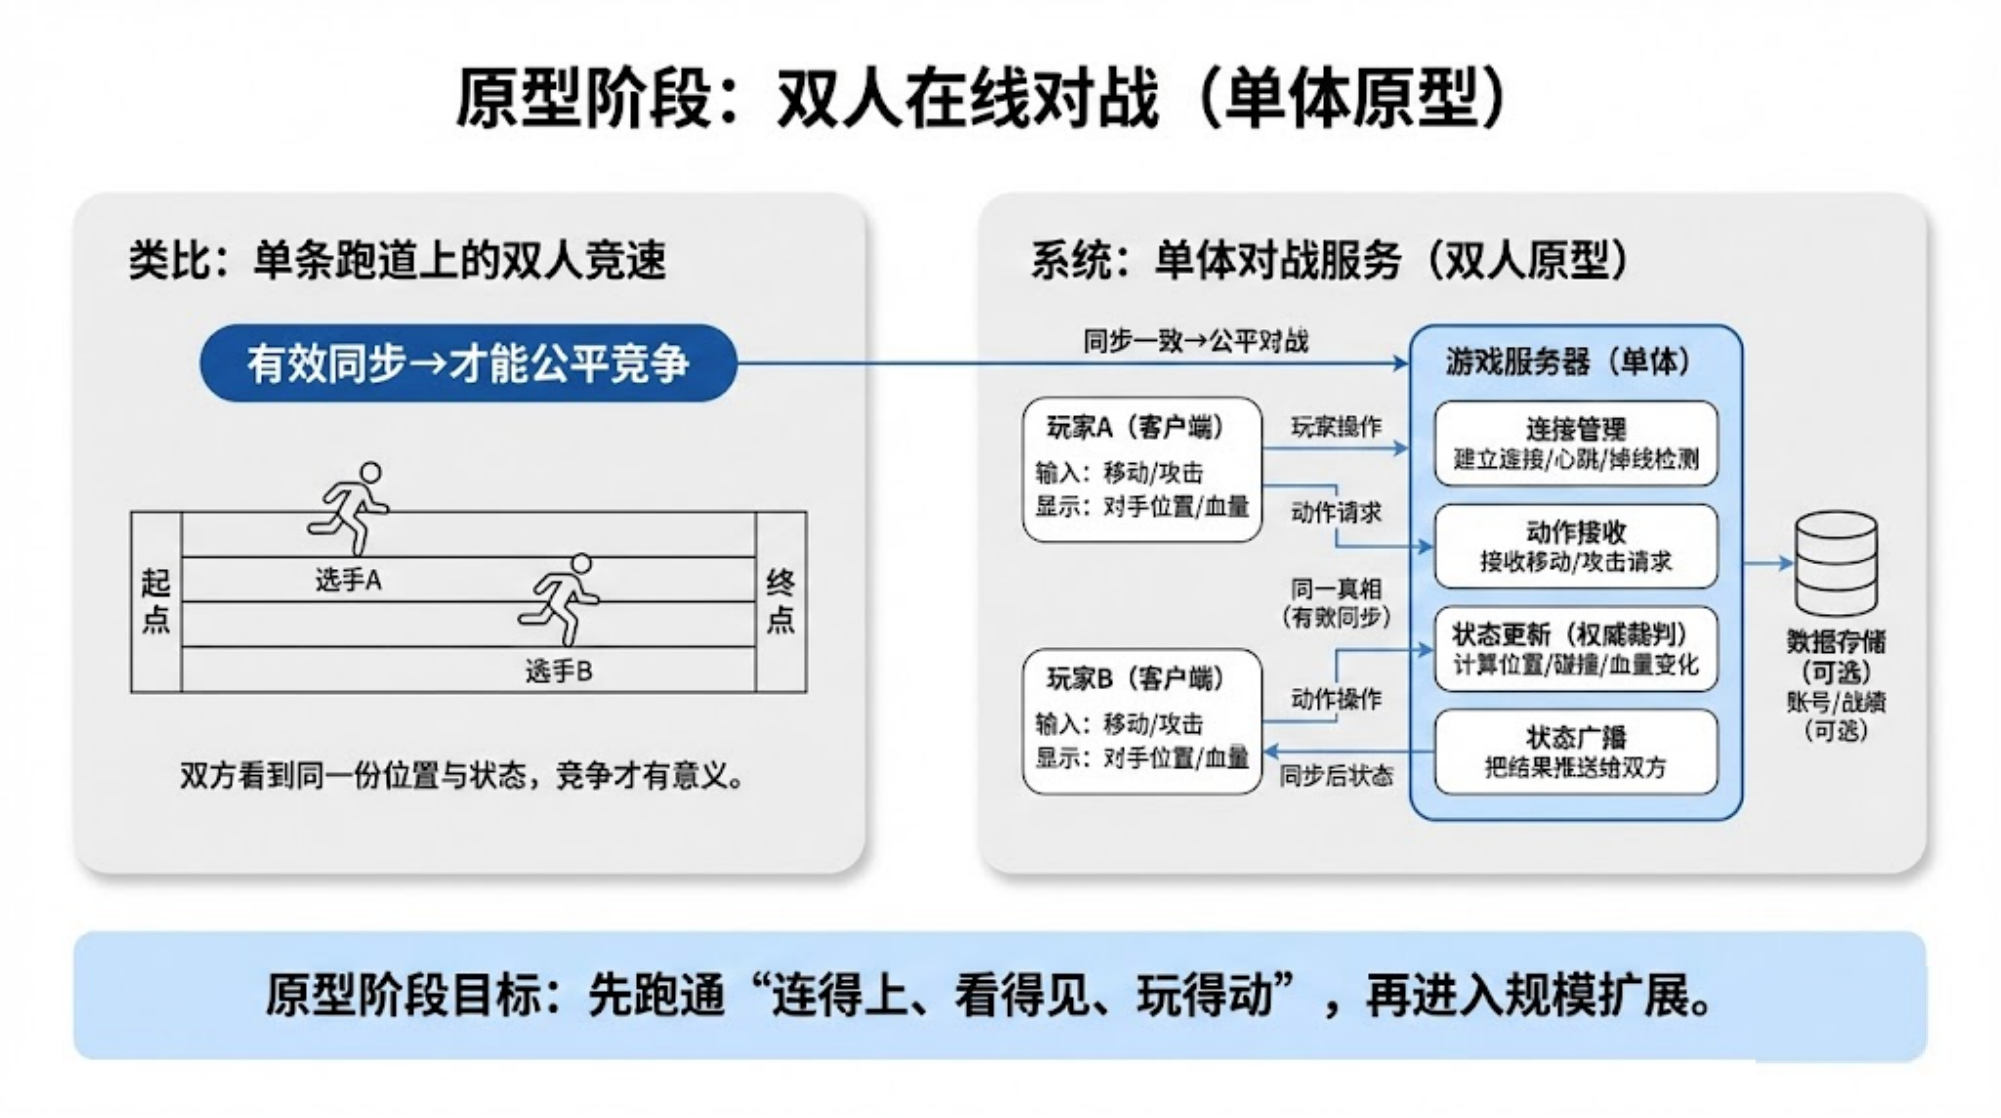
\includegraphics[width=1.0\textwidth]{figures/intro-phase2.png}
%     \vspace{-30pt}
%     \caption{可竞技的单条跑道与单体架构}
%     \label{fig:intro-phase2}
%     \vspace{-15pt}
% \end{figure*}

% 如图\ref{fig:intro-phase2}所示，\textbf{原型阶段}的目标是先构建一个最基础在线对战系统。我们基于最典型的“双人同图对局”开始游戏：两位玩家进入同一张地图开始走位、试探，每一次操作都应当在对方视角中及时出现并得到一致的反馈。若双方看到的位置、血量或判定结果不一致，就会立刻产生“我明明打中了/我明明躲开了”的割裂体验，对战也就失去可信的基础。因此，这一阶段关注的核心不是玩法的复杂度，而是把小地图的实时交互闭环跑通，并确保双方始终基于同一份游戏状态进行对抗。

% 在系统实现层面，我们用一个单体游戏服务器来支撑这一基本闭环。客户端发出动作请求，服务端负责管理连接、接收请求、计算新的游戏状态，并将结果广播回每个客户端。服务器的状态广播就像比赛中的裁判，它确保每一方看到的是相同的状态，从而让两位玩家在游戏过程中感受到实时、可信的反馈。只有把连接、请求、状态更新与同步三个步骤完整跑通，才能保证玩家能“连得上、看得见、玩得动”，为后续面对更多玩家或更复杂业务的扩展打下最基本的工程基础。

% 进入\textbf{并发优化阶段}后，如图\ref{fig:intro-phase3}所示，交互场景发生了质变：战场不再局限于双人对决，而是瞬间涌入成百上千名玩家。这种高密度的交互使得原有的架构不堪重负，由此产生的操作延迟感、动作变形感会迅速消耗玩家的耐心。映射到系统层面，就是处理请求的速度跟不上玩家请求数的增长，导致卡顿、延迟甚至错误。因此，本阶段的核心任务是精准定位瓶颈，通过在现有架构下进行精细化调优，拓展系统的承载极限，使其在多用户高压环境下依然能保持高效与稳定。

% \begin{figure*}[htbp]
%     \vspace{-13pt}
%     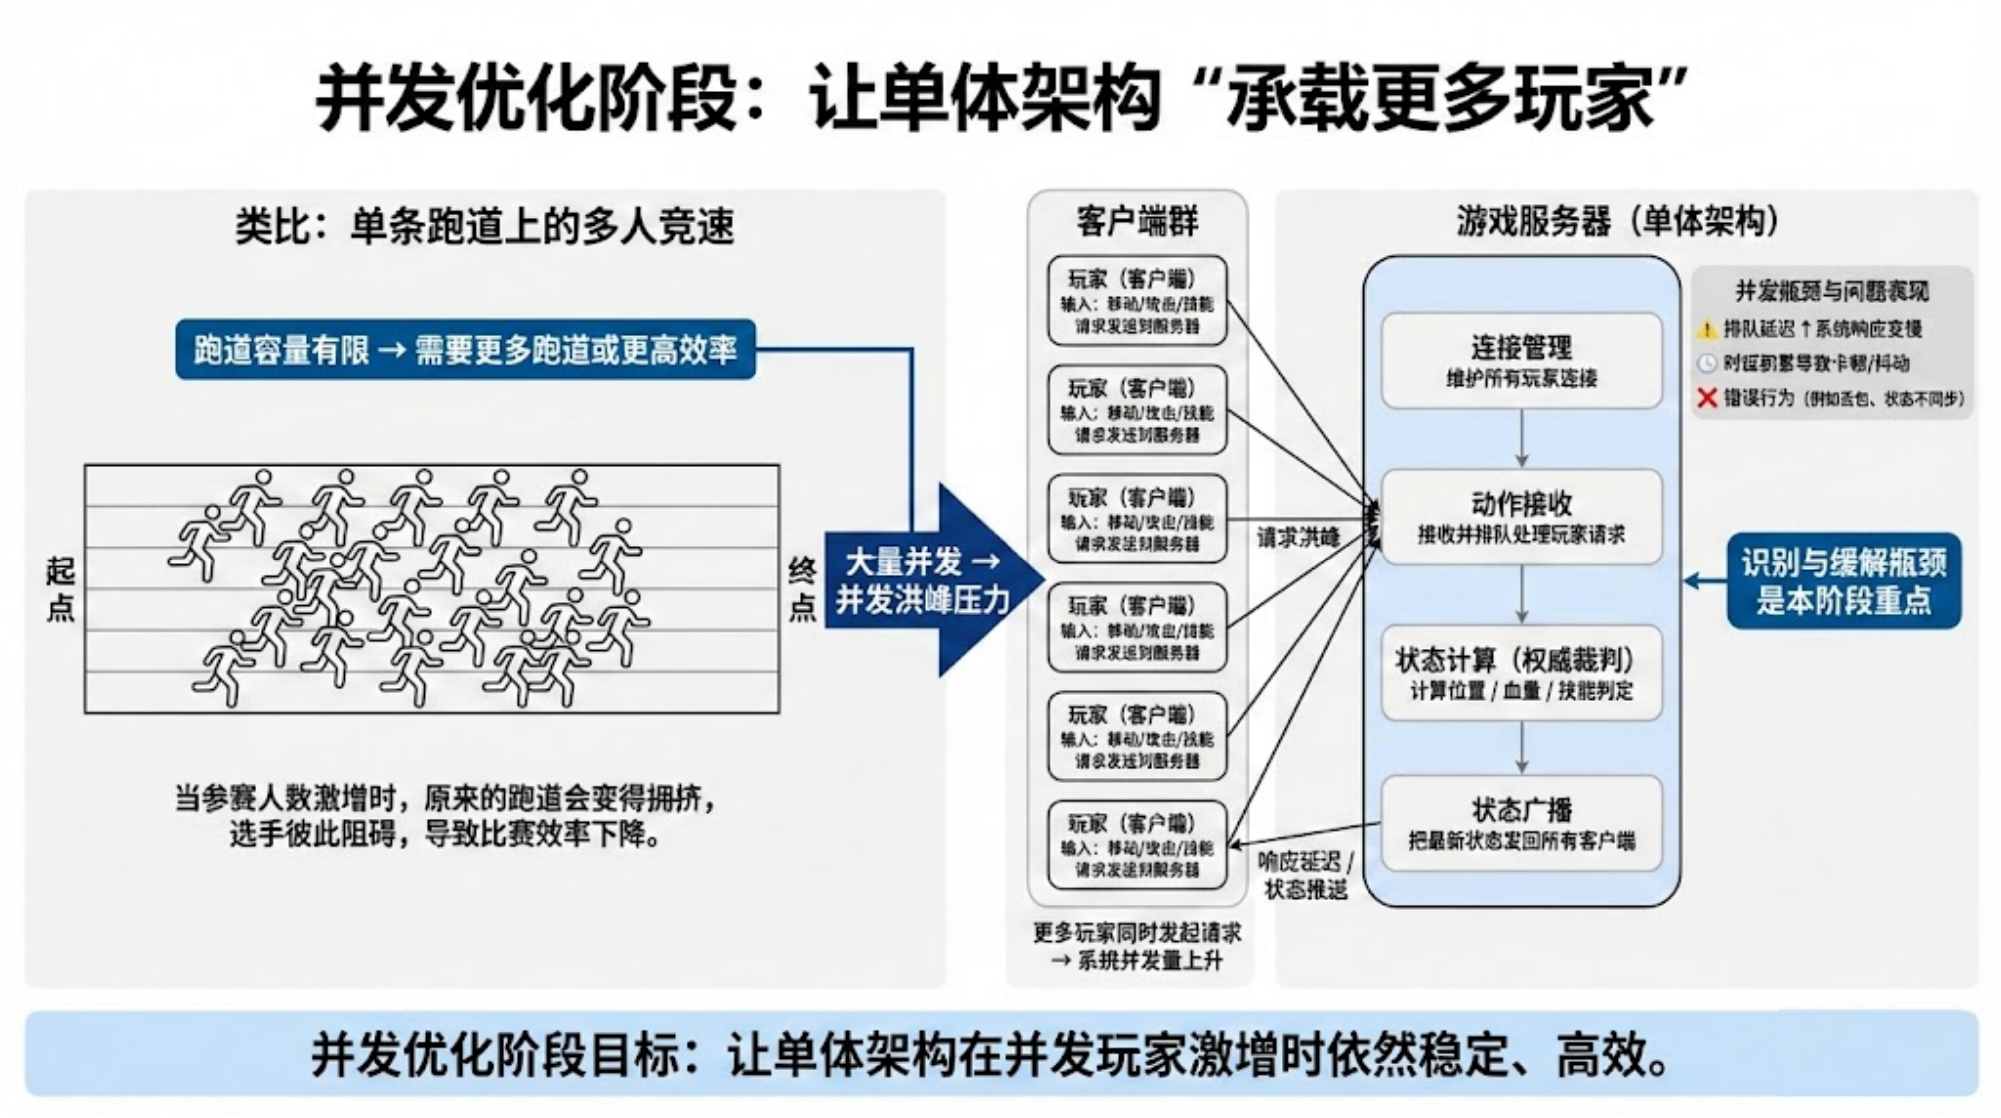
\includegraphics[width=1.0\textwidth]{figures/intro-phase3.png}
%     \vspace{-30pt}
%     \caption{高性能的单条跑道与并发单体架构}
%     \label{fig:intro-phase3}
%     \vspace{-15pt}
% \end{figure*}

% 如图\ref{fig:intro-phase4}所示，当同一张地图里的玩家数量持续激增，“把所有人都塞进一张地图”的策略终究会遇到天花板。战场越拥挤，每一次移动或技能释放所引发的同步成本就越高，最终导致系统不堪重负。为了承载更大的规模，我们必须打破单体限制，将在线世界开辟成由多张地图组成的“互联群岛”，这标志着我们正式进入了\textbf{分布式阶段}。在系统中，这意味着将不同功能拆分到多台机器上协同运行，各自处理特定的任务（如登录、对战逻辑、状态同步等），并通过网络协调它们之间的状态一致。对应到系统设计，这意味着不再由一台机器包揽所有工作，而是将登录、逻辑计算、状态同步等任务拆分到不同的机器上协同处理。虽然这种“人多力量大”的模式解决了容量难题，但也带来了挑战：多地图之间如何保持步调一致？如何防止某张地图突然崩溃导致整个游戏不可玩？因此，本阶段我们将以游戏中的跨地图互动为例，带读者理解分布式系统中“协同”与“一致性”的本质，并动手解决这些问题。

% \begin{figure*}[htbp]
%     \vspace{-13pt}
%     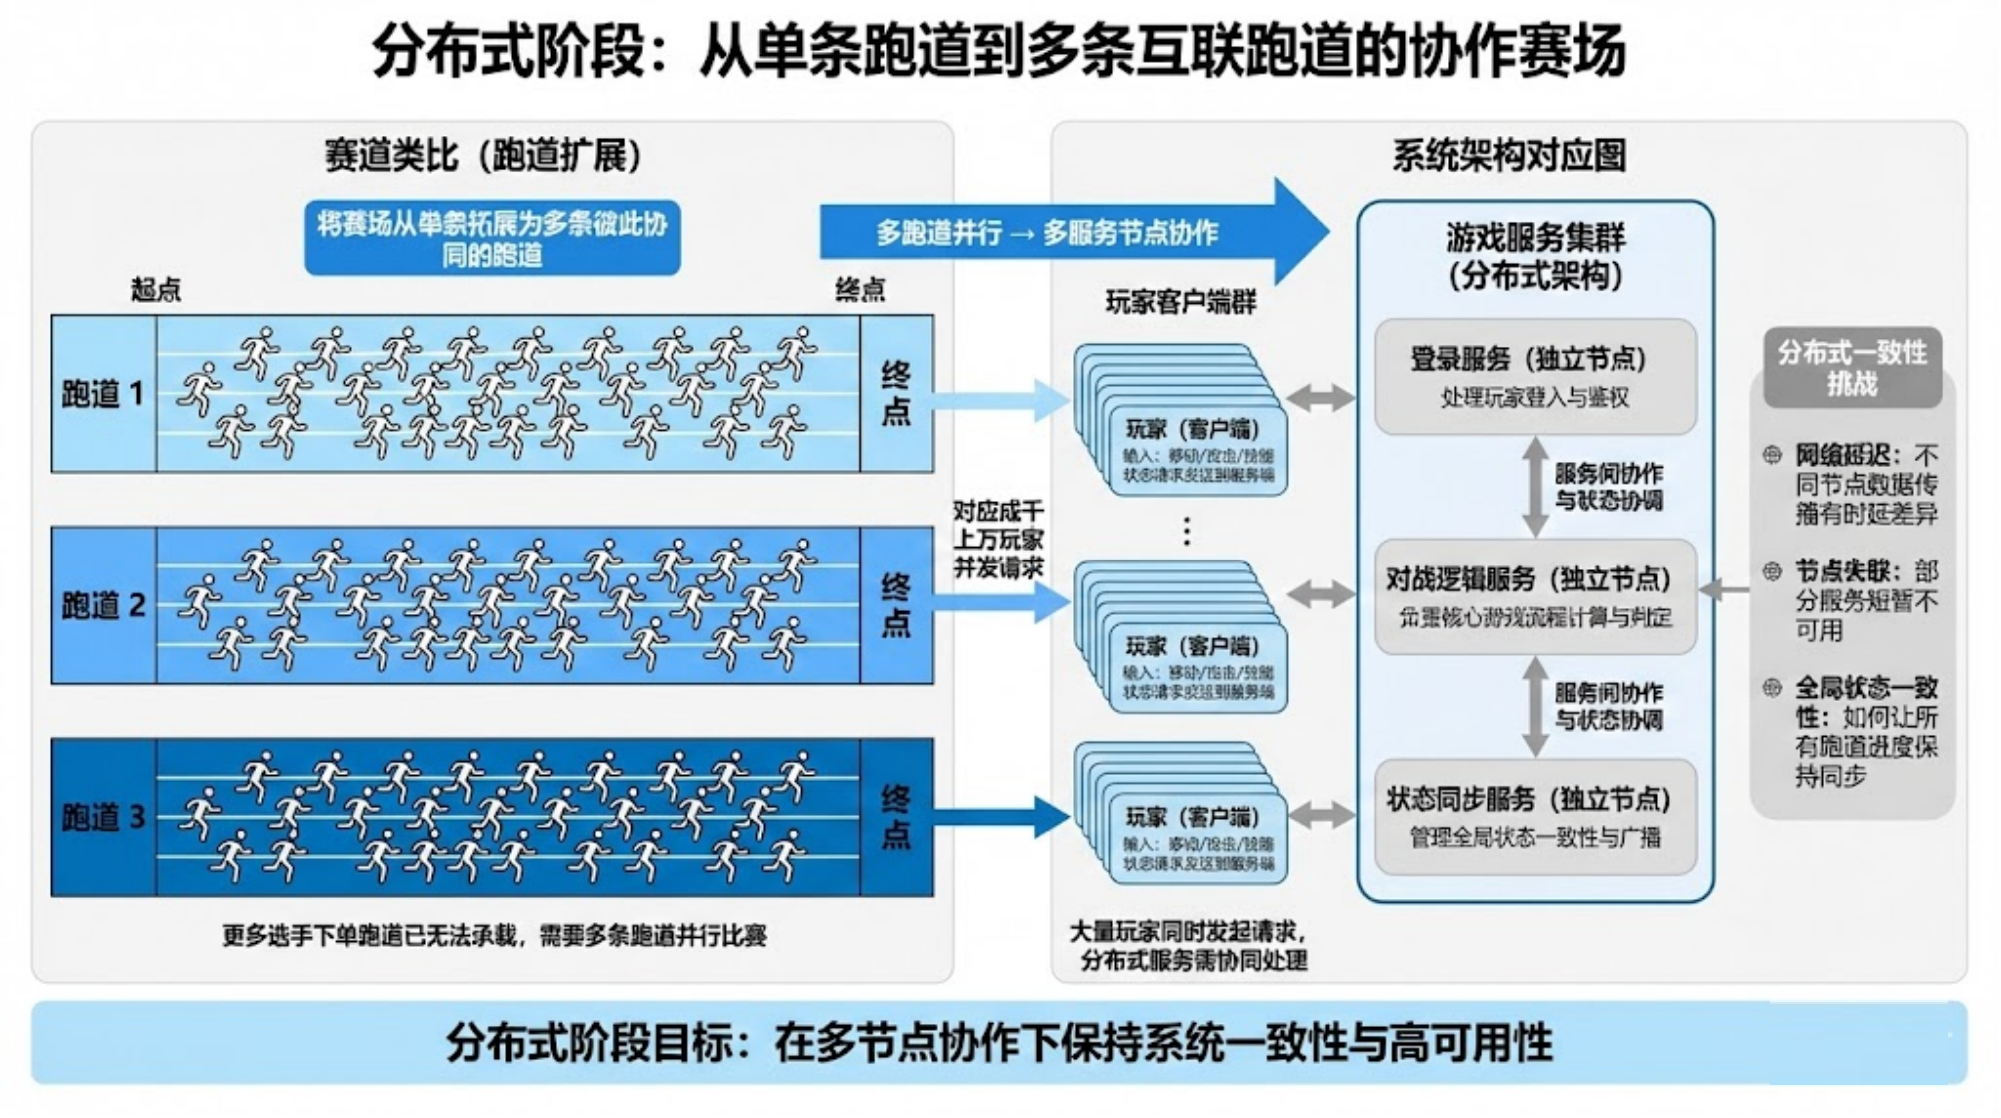
\includegraphics[width=1.0\textwidth]{figures/intro-phase4.png}
%     \vspace{-30pt}
%     \caption{多跑道与多服务器分布式架构}
%     \label{fig:intro-phase4}
%     \vspace{-15pt}
% \end{figure*}

% 最终，在\textbf{容器化阶段}，如图\ref{fig:intro-phase5}所示，我们的视角不再局限于手动管理地图，而是升级为对整个“游戏宇宙”的自动化治理。这种能力类似于智能化的副本管理系统：它不再依赖人工去开服合服，而是将服务打包成一个个标准的副本单元（容器）。当玩家蜂拥而至时，系统能瞬间复制出成百上千个平行的副本世界来承载流量；当人潮退去，多余的副本则会被自动回收。对应到技术层面，这正是容器打包与自动化编排的精髓，通过将服务标准化封装，配合编排系统（如Kubernetes）的调度，系统能够根据实时用户数量动态伸缩资源，甚至在某个副本“崩溃”时毫秒级自动重建，无需人工连夜上线救火。这种弹性调度与自动化管理，正是云计算支撑大规模复杂业务的基石。

% \begin{figure*}[htbp]
%     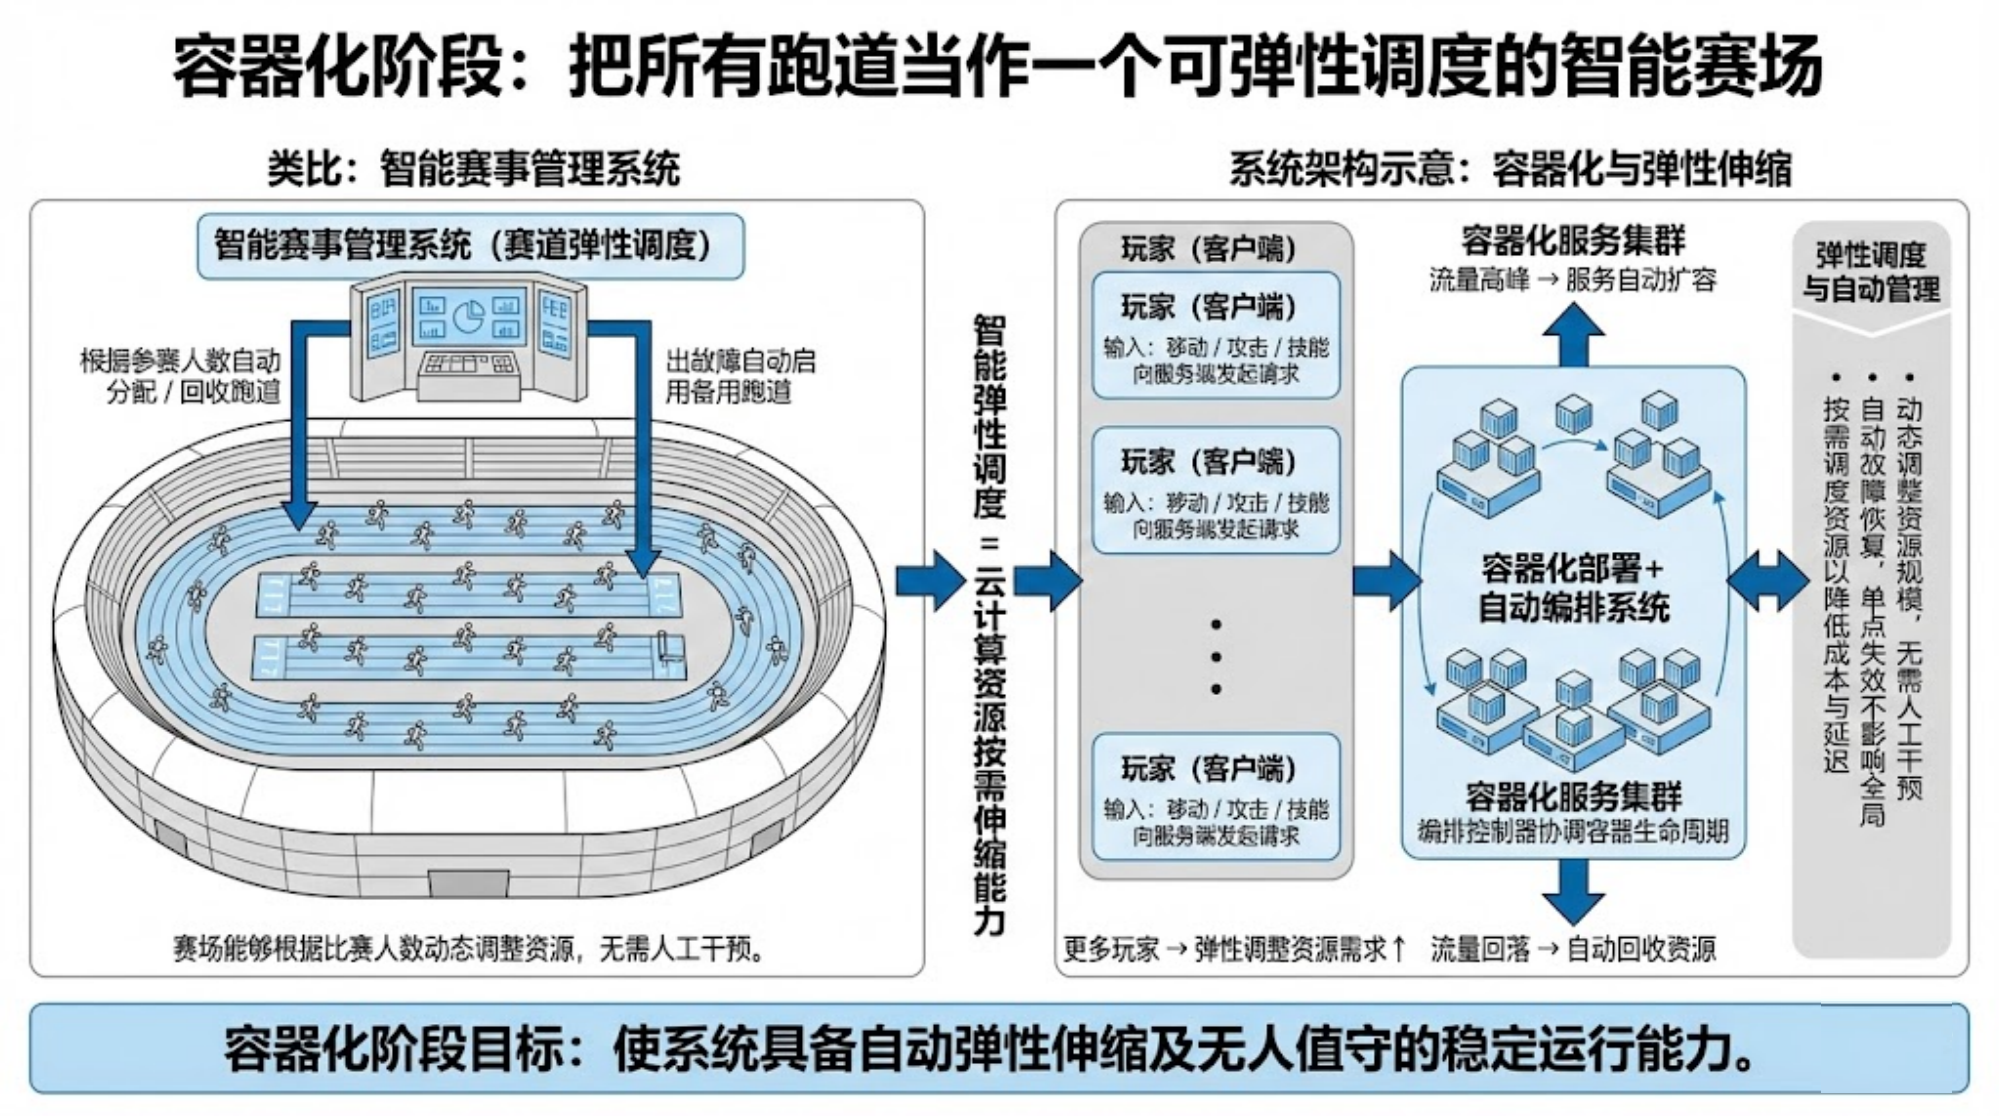
\includegraphics[width=1.0\textwidth]{figures/intro-phase5.png}
%     \vspace{-30pt}
%     \caption{弹性智能体育场与容器化架构}
%     \label{fig:intro-phase5}
%     \vspace{-15pt}
% \end{figure*}

% 通过梳理这一系列从单张小地图到分布式群岛，再到弹性平行世界的架构演进，读者不仅能直观地看到系统在不同规模下所面临的特定瓶颈，更能深刻理解每一项技术引入背后的工程必然性。这套演进逻辑清晰地揭示了云计算的核心原理：我们何时需要深挖单机性能，何时必须转向横向协作，又在何种契机下引入弹性扩缩与自动化编排。正是这些能力的层层递进与有机结合，最终支撑起大规模在线服务的稳定运行。
